\usetikzlibrary{arrows}
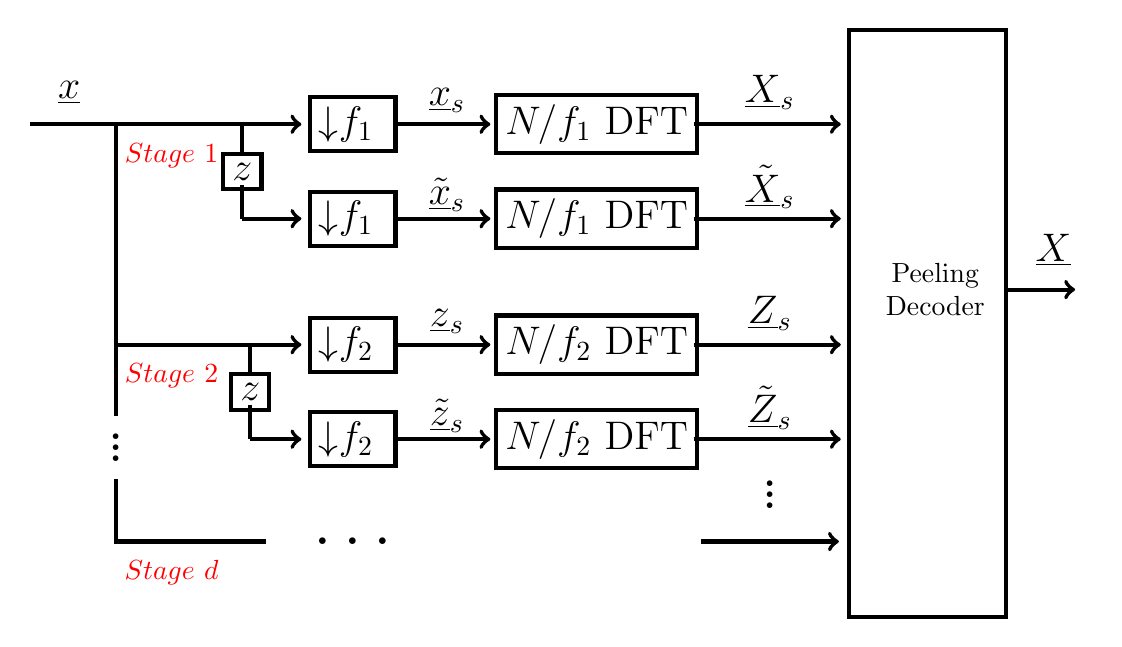
\begin{tikzpicture}

 % Downsampling blocks
\node[draw,align=center,thick,line  width =1.5pt] at (1,5.1) {\Large{$\mathbf{\downarrow} f_2$} };
\node[draw,align=center,thick,line  width =1.5pt] at (1,6.3) {\Large{$\mathbf{\downarrow} f_2$ }};

\node[draw,align=center,thick,line  width =1.5pt] at (1,7.9) {\Large{$\mathbf{\downarrow} f_1$} };
\node[draw,align=center,thick,line  width =1.5pt] at (1,9.1) {\Large{$\mathbf{\downarrow} f_1$ }};

%  Input lines to the down-sampling block
 \draw[->,thick,line  width =1.5pt] (-0.3,5.1) -- (0.35,5.1);
 \draw[->,thick,line  width =1.5pt] (-0.3,6.3) -- (0.35,6.3);
  
 \draw[->,thick,line  width =1.5pt] (-0.4,7.9) -- (0.35,7.9);
 \draw[->,thick,line  width =1.5pt] (-0.4,9.1) -- (0.35,9.1);

%  Delay blocks
\node[draw,align=center,thick,line  width =1.5pt] at (-0.3,5.7) {\Large{$z$}};
\node[draw,align=center,thick,line  width =1.5pt] at (-0.4,8.5) {\Large{$z$}};

% paths connecting the delay blocks
 \draw[thick,line  width =1.5pt] (-0.3,5.1) -- (-0.3,5.53);
 \draw[thick,line  width =1.5pt] (-0.3,5.9) -- (-0.3,6.3);
 
 \draw[thick,line  width =1.5pt] (-0.4,7.9) -- (-0.4,8.33);
 \draw[thick,line  width =1.5pt] (-0.4,8.7) -- (-0.4,9.1);
 
% paths connecting the two stages   
 \draw[thick,line  width =1.5pt] (-0.4,9.1) -- (-2,9.1);
 \draw[thick,line  width =1.5pt] (-0.3,6.3) -- (-2,6.3);
 \draw[thick,line  width =1.5pt] (-2,6.3) -- (-2,9.1);
  \draw[thick,line  width =1.5pt] (-3.1,9.1) -- (-2,9.1);
  \draw[thick,line  width =1.5pt] (-2,6.3) -- (-2,5.4);
  
  
  % DFT blocks
\node[draw,align=center,thick,line  width =1.5pt] at (4.1,5.1) {\Large{$N/f_2$ DFT}};
\node[draw,align=center,thick,line  width =1.5pt] at (4.1,6.3) {\Large{$N/f_2$ DFT}};

\node[draw,align=center,thick,line  width =1.5pt] at (4.1,7.9) {\Large{$N/f_1$ DFT}};
\node[draw,align=center,thick,line  width =1.5pt] at (4.1,9.1) {\Large{$N/f_1$ DFT}};

% Connectors
 \draw[->,thick,line  width =1.5pt] (1.55,9.1) -- (2.75,9.1);
 \draw[->,thick,line  width =1.5pt] (1.55,7.9) -- (2.75,7.9);
  
 \draw[->,thick,line  width =1.5pt] (1.55,6.3) -- (2.75,6.3);
 \draw[->,thick,line  width =1.5pt] (1.55,5.1) -- (2.75,5.1);

 \draw[->,thick,line  width =1.5pt] (5.33,9.1) -- (7.2,9.1);
 \draw[->,thick,line  width =1.5pt] (5.33,7.9) -- (7.2,7.9);
 
 \draw[->,thick,line  width =1.5pt] (5.33,6.3) -- (7.2,6.3);
 \draw[->,thick,line  width =1.5pt] (5.33,5.1) -- (7.2,5.1);
 
 
  % Labels
  \node[draw=none,align=center] at (-2.6,9.5) {\Large{$\underline{x}$}};
  
  \node[draw=none,align=center] at (2.2,9.4) {\Large{$\underline{x}_{s}$}};
  \node[draw=none,align=center] at (2.2,8.2) {\Large{$\underline{\tilde{x}}_{s}$}};
  \node[draw=none,align=center] at (2.2,6.6) {\Large{$\underline{z}_{s}$}};
  \node[draw=none,align=center] at (2.2,5.4) {\Large{$\underline{\tilde{z}}_{s}$}};
  
  \node[draw=none,align=center] at (6.3,9.5) {\Large{$\underline{X}_{s}$}};
  \node[draw=none,align=center] at (6.3,8.3) {\Large{$\underline{\tilde{X}}_{s}$}};
  \node[draw=none,align=center] at (6.3,6.7) {\Large{$\underline{Z}_{s}$}};
  \node[draw=none,align=center] at (6.3,5.5) {\Large{$\underline{\tilde{Z}}_{s}$}};
  
  \node [draw=none] at (-2,5.1) {\Huge${\vdots}$} ;
  
   \node[draw=none,align=center] at (-1.3,8.7) {\color{red}$Stage ~1$};
  \node[draw=none,align=center] at (-1.3,5.9) {\color{red}$Stage ~2$};
   \node[draw=none,align=center] at (-1.3,3.4) {\color{red}$Stage ~d$};
\draw [thick,line  width =1.5pt](-2,4.6) -- (-2,3.8) -- (-0.1,3.8) ;
 \node[draw=none,align=center] at (1,3.8) {\Huge${\ldots}$};
 
\draw [thick,line  width =1.5pt] (7.3,2.8424) rectangle (9.3,10.3);
\node (v1) at (5.3,3.8) {};
\node (v2) at (7.3,3.8) {};
\draw  [->,thick,line  width =1.5pt](v1) edge (v2);
\node at (6.3,4.5) {\Huge${\vdots}$};
\node [text width=3cm, align =center ] at (8.4,7) {Peeling \\ Decoder};
\node (v3) at (9.2,7) {};
\node (v4) at (10.3,7) {};
\draw [thick, ->,line  width =1.5pt] (v3) edge (v4);
\node at (9.9,7.5) {\Large{$\underline{X}$}};
\end{tikzpicture}